\documentclass[11pt,letterpaper]{article}
\usepackage[lmargin=1in,rmargin=1in,tmargin=1in,bmargin=1in]{geometry}
\usepackage{../style/homework}
\usepackage{../style/commands}
\setbool{quotetype}{true} % True: Side; False: Under
\setbool{hideans}{true} % Student: True; Instructor: False

% -------------------
% Content
% -------------------
\begin{document}

\homework{18: Due 01/19}{Probability theory is nothing but common sense reduced to calculation.}{Pierre-Simon Laplace}

% Problem 1
\problem{10} Consider the curve $C(x)$ given below. \par
	\[
	\fbox{
	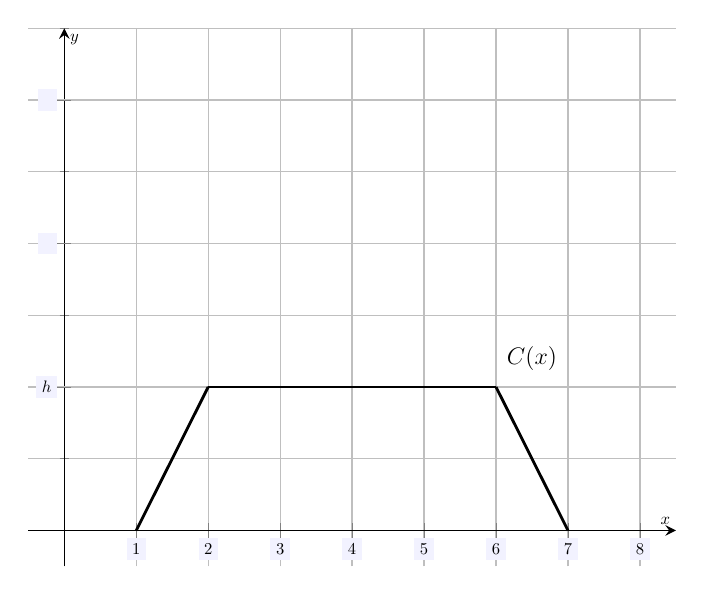
\begin{tikzpicture}[scale=1.2,every node/.style={scale=0.5}]
	\begin{axis}[
	grid=both,
	axis lines=middle,
	ticklabel style={fill=blue!5!white},
	xmin= -0.5, xmax=8.5,
	ymin= -0.25, ymax=3.5,
	xtick={1,2,...,8},
	ytick={},
	%ymajorticks=false,
	extra y ticks={1,2,3},
	extra y tick labels={$h$,\phantom{2},\phantom{3}},
	minor x tick num = 0,
	minor y tick num = 1,
	xlabel=\(x\),ylabel=\(y\),
	]
	\node at (6.5,1.2) {\Large$C(x)$};
	\addplot[domain=1:2,samples=2,line width=0.03cm] (x, x - 1);
	\addplot[domain=2:6,samples=2,line width=0.03cm] (x, 1);
	\addplot[domain=6:7,samples=2,line width=0.03cm] (x, 7 - x);

	\end{axis}
	\end{tikzpicture}
	}
	\] \par

\begin{enumerate}[(a)]
\item Find the value of $h$ that makes $C(x)$ a density curve. 
\item Find $P(x \leq 3)$. 
\end{enumerate} 



\newpage



% Problem 2
\problem{10} Suppose Mork and Mindy are both underpaid workers. Mork's job has salaries that follow a distribution with mean \$52,000 and standard deviation \$6,000 but Mork himself makes \$41,000. Mindy's job has a salary distribution with mean \$88,000 and standard deviation \$3,000 and Mindy makes \$75,000. Assume both company's salaries are normally distributed. Compared to other workers at their company, who makes less? Explain. 



\newpage



% Problem 3
\problem{10} Suppose that a random variable, $X$, is drawn from a normal distribution with mean 22.7 and standard deviation 5.1. Compute the following:
	\begin{enumerate}[(a)]
	\item $P(X= 22.7)$
	\item $P(X \leq 18)$
	\item $P(X > 30)$
	\item $(18 \leq X \leq 30)$
	\end{enumerate}



\newpage



% Problem 4
\problem{10} Suppose the exam scores for a college entrance exam were normally distributed with mean 74 and standard deviation 6.2. What is the minimal score a student needs to be in the top 10\% of exam takers? 



\newpage



% Problem 5
\problem{10} Watch Stand-Up Math's ``How to estimate a population using statisticians'' on YouTube. Being as detailed as possible, comment on what you learned and how it relates to the course material. 


\end{document}